\section{Second dataset: EMPIAR-10491}
\label{sec:suppl:dataset2}

\paragraph{Data.}
We repeat the fixed-pose comparison on purified human apoferritin (EMPIAR-10491, octahedral symmetry O), using the five tilt series of WarpTools' end-to-end example (TS\_1, 11, 17, 23 and 32; 41 tilts each, 0.7894\,\AA/px, 2.64\,e$^-$/\AA$^2$ per tilt).
% src: runs/dataset10491_20261121/reference_e2e.sh (warpem/warp scripts/EMPIAR-10491_5TS_e2e.sh: --angpix 0.7894, --exposure 2.64); runs/dataset10491_20261121/raw/verify.txt (205 frame files + gain, sizes equal to the server's); runs/dataset10491_20261121/raw/mdoc/TS_*.mrc.mdoc (41 SubFramePath entries each)

\paragraph{Preprocessing.}
WarpTools 2.0.0dev33 follows that example: frame motion and CTF, patch tracking in IMOD, tilt-series CTF, tomograms at 10\,\AA/px and template matching against EMD-15854 (O, 130\,\AA).
% src: runs/dataset10491_20261121/03_warp.sh; runs/dataset10491_20261121/logs/02_warp_install.log (warp-2.0.0dev33); runs/dataset10491_20261121/RUNLOG.txt
The defocus-handedness check gives an average correlation of $+0.843$, so the handedness is kept.
% src: runs/dataset10491_20261121/logs/warp_ts_defocus_hand_check.log (Average correlation: 0.843; 'no flip'); RUNLOG.txt (decision --set_noflip)
Thresholding the matches at 6 standard deviations keeps 1,466 of 2,608 picks; the 1,461 particles visible in all 41 tilts are exported as 2D particle series, at 4\,\AA/px (box 64) and at 1.5788\,\AA/px (box 128).
% src: runs/dataset10491_20261121/logs/warp_threshold_picks.log (2608 particles found, 1466 left); runs/dataset10491_20261121/logs/relion_relion_input.log (1461 particles, 0 with an invisible frame; export --max_missing_tilts 0)
RELION-5.0.1 builds a de novo initial model at 4\,\AA/px and refines it at 1.5788\,\AA/px with random half-sets (765 and 696 particles); auto-refine converges after 23 iterations.
% src: runs/dataset10491_20261121/04_relion.sh (options of the example; --sym O); runs/dataset10491_20261121/stags/roundtrip_A/warp_roundtrip.txt (half-sets 765 / 696); runs/dataset10491_20261121/logs/relion_refine3d.log (converged; last iteration file run_it023)
Its gold-standard resolution after post-processing is 4.59\,\AA\ (B-factor $-119$\,\AA$^2$).
% src: runs/dataset10491_20261121/warp/relion/PostProcess/job004/postprocess.star (_rlnFinalResolution 4.592873, _rlnBfactorUsedForSharpening -118.80488)
The soft mask is thresholded at the value that encloses the expected volume of the 24-mer (506\,kDa at 1.21\,\AA$^3$/Da) in the 15\,\AA\ low-passed consensus map, then extended by 3 and softened over 6 pixels.
% src: runs/dataset10491_20261121/warp/relion/MaskCreate/job003/threshold.json (mass_Da 506400, threshold 0.004577 = 1.99 SD above the mean)
We stop before M, the multi-particle refinement with which the example reaches about 3\,\AA, so this dataset tests the maps at 8--4.5\,\AA.
% src: runs/dataset10491_20261121/reference_e2e.sh (MCore steps, comments '# 3.0 A' / '# 2.9 A')

\paragraph{Fixed-pose protocol.}
As in \mainref{sec:results:efficiency}, RELION's refined poses, optics and mask are fixed, and each half-set is reconstructed twice: as a voxel map and as a Gaussian map fitted to its tilt images.
Here every particle of the half-set is used (765 and 696) rather than 250-particle subsets, at the export's sampling of 1.5788\,\AA/px.
% src: runs/dataset10491_20261121/stags/fit_h1/summary.txt (765 particles, box 128 at 1.579 A/px); runs/dataset10491_20261121/stags/fit_h2/summary.txt (696 particles)
The voxel map is our Wiener reconstruction of the same particles, not RELION's; at RELION's poses it reproduces RELION's unfiltered map of the same half-set with FSC 0.9999 at 8\,\AA\ in both halves.
% src: runs/dataset10491_20261121/stags/roundtrip.json (gate pass; fsc_same_half_8A 0.99990 / 0.99986; relion5 true; confirmation pass)
The Gaussian map has 48,000 Gaussians (2,000 per asymmetric unit) and is fitted for 32 passes (4,080 and 3,712 iterations of 6 particles), with the Fourier renderer, whitened loss, and the density outside the mask subtracted from the images using the voxel map of the same particles.
% src: runs/dataset10491_20261121/stags/fit_h1/fit-config.json and fit_h2/fit-config.json; runs/dataset10491_20261121/05_stags.sh (fit_half: --K 48000 --batch 6 --renderer fourier --whiten 1 --subtract_outside 1 --bin 1); runs/dataset10491_20261121/logs/stags_fit_h1.log (iterations 4080), stags_fit_h2.log (3712)
Fitting both maps of a half-set takes 12.0 and 11.0\,min on one RTX 4090 per half, of which the Gaussian fit takes 514 and 475\,s.
% src: runs/dataset10491_20261121/logs/stags_fit_h1.log ('done in 12.0 min'; 'B ray ... [514s'), stags_fit_h2.log ('done in 11.0 min'; 'B ray ... [475s')
Unlike the main study, which scores at 6.5--5.6\,\AA, we report the FSC 0.143 crossing against the opposite RELION half map inside RELION's mask, and the FSC at fixed resolutions (\cref{tab:suppl:dataset2,fig:suppl:dataset2}).

\begin{table}[t]
\centering
\footnotesize
\setlength{\tabcolsep}{3pt}
\resizebox{\columnwidth}{!}{\begin{tabular}{@{}lccccc@{}}
\toprule
& \multicolumn{2}{c}{Crossing (\AA) $\downarrow$} & \multicolumn{3}{c}{FSC at $\uparrow$} \\
\cmidrule(lr){2-3}\cmidrule(lr){4-6}
& 0.143 & 0.5 & 8\,\AA & 6\,\AA & 4.5\,\AA \\
\midrule
% src: runs/dataset10491_20261121/stags/score_B/results.json (pairs cross_h1 / cross_h2: crossings_A.mask_corrected, fsc_at); runs/dataset10491_20261121/supp_dataset2_numbers.json (gaussian)
Gaussian & 4.54 / 4.62 & 5.92 / 6.05 & 0.904 / 0.903 & 0.543 / 0.467 & 0.114 / 0.151 \\
% src: runs/dataset10491_20261121/stags/score_A/results.json (pairs cross_h1 / cross_h2); runs/dataset10491_20261121/supp_dataset2_numbers.json (voxel)
Voxel & 4.52 / 4.51 & 6.01 / 6.02 & 0.887 / 0.888 & 0.493 / 0.491 & 0.136 / 0.139 \\
% src: runs/dataset10491_20261121/stags/score_B/results.json (pair relion_gold; identical in score_A: supp_dataset2_numbers.json relion_gold_identical_in_A true)
RELION-5 & 4.50 & 6.00 & 0.888 & 0.499 & 0.143 \\
\bottomrule
\end{tabular}}
\caption{\textbf{EMPIAR-10491 at fixed RELION-5 poses.} Mask-corrected FSC of the half-1 / half-2 maps against the opposite RELION-5 half map; RELION-5: its own half 1 against half 2. Same particles, poses, mask and scorer for every row.}
\label{tab:suppl:dataset2}
\end{table}

\begin{figure}[t]
\centering
% src: fig/supp_dataset2_fsc.pdf by scripts/paper_supp_dataset2.py (branch supp-10491); curves: runs/dataset10491_20261121/stags/score_B/results.json (Gaussian, RELION-5 half 1 vs 2) and runs/dataset10491_20261121/stags/score_A/results.json (voxel), pairs cross_h1, cross_h2, relion_gold, mask_corrected
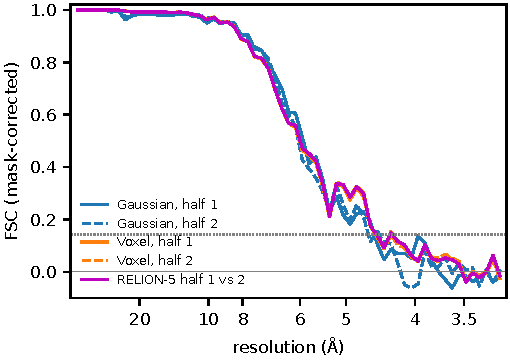
\includegraphics[width=\columnwidth]{fig/supp_dataset2_fsc.pdf}
\caption{\textbf{EMPIAR-10491 FSC.} Gaussian (blue) and voxel (orange) half 1 (solid) / 2 (dashed) vs.\ opposite RELION-5 half; RELION-5 half 1 vs.\ 2 (magenta). Mask-corrected.}
\label{fig:suppl:dataset2}
\end{figure}


\paragraph{Results.}
At 8 and 6\,\AA\ the Gaussian maps agree better with the opposite RELION half map than the voxel maps do (0.904/0.903 against 0.887/0.888 at 8\,\AA; 0.543/0.467 against 0.493/0.491 at 6\,\AA), except for half~2 at 6\,\AA.
% src: runs/dataset10491_20261121/supp_dataset2_numbers.json (gaussian / voxel fsc_at 8, 6)
At the resolution limit they do not: the Gaussian maps cross 0.143 at 4.54/4.62\,\AA, the voxel maps at 4.52/4.51\,\AA, and RELION's own half maps at 4.50\,\AA.
% src: runs/dataset10491_20261121/stags/score_B/results.json, score_A/results.json (crossings_A.mask_corrected 0.143: 4.535 / 4.624, 4.516 / 4.511, relion_gold 4.501)
The voxel maps essentially reproduce RELION's FSC, and the Gaussian maps trail them by 0.02 and 0.11\,\AA.
On this dataset, therefore, the Gaussian map matches the voxel map from the same particles at the crossing, with a gain at 8--6\,\AA\ but no gain in resolution.
The two Gaussian half maps agree with each other well beyond their crossings (FSC 0.29 at 3.5\,\AA, where each scores about 0 against RELION), which is the shared-basis correlation of \cref{sec:suppl:eval}; we therefore score only against RELION's half maps.
% src: runs/dataset10491_20261121/supp_dataset2_numbers.json (gaussian_own_gold fsc_at 3.5 0.286, crossing_0143 null; gaussian fsc_at 3.5 -0.014 / 0.014)
RELION's post-processed 4.59\,\AA\ and the 4.50\,\AA\ of our scorer come from the same half maps and mask; they differ in how the curve is mask-corrected (RELION randomizes phases beyond 8.08\,\AA, our scorer beyond 20\,\AA) and read off.
% src: runs/dataset10491_20261121/warp/relion/PostProcess/job004/postprocess.star (4.592873); runs/dataset10491_20261121/logs/relion_postprocess.log ('randomize phases beyond: 8.08346 Angstroms'); runs/dataset10491_20261121/stags/score_B/results.json (phase_randomization cutoff_A 20.0; relion_gold 4.501; inputs.mask = MaskCreate/job003/mask.mrc)

\paragraph{Limitations.}
The poses come from RELION and are not refined, so this isolates the map representation, as in the main fixed-pose study, and says nothing about end-to-end refinement on this dataset.
The comparison is reference-assisted: the mask comes from RELION's consensus map, the Wiener constant of each voxel map is the best of four by its score against the opposite RELION half (0.05 and 0.2), and the Gaussian maps' contrast sign is set against that half map at 40--12\,\AA.
% src: runs/dataset10491_20261121/stags/fit_h1/results.json, fit_h2/results.json (subsets[0].A_best_wiener 0.05 / 0.2; contrast_sign); runs/dataset10491_20261121/stags/fit_h1/run.log ('contrast: sign +1 (mean FSC 40-12 A vs reference')
It is one dataset size (1,461 particles from five tilt series), one fit per half and one random seed, without the per-tilt-series alignment refinement of M, so its resolution stays at about 4.5\,\AA, and we have no estimate of run-to-run variation of the crossings.
